% Appendix companion to Section 5. Setup, seed variability, and the three
% parameter sweeps (evidence budget, training fraction, encoder input length),
% each with its figure, protocol note and the bounds on what it licenses.

\subsection{Setup}
\label{app:setup}

\paragraph{Splits.}
The split is a date-ordered $13{,}815/3{,}944/3{,}352$ partition of the
$21{,}111$ idea-level samples in \textsc{IdeaDelta}.

\paragraph{Configuration.}
All runs share one configuration and vary a single parameter at a time:
\texttt{deberta-v3-base} backbone, 8 epochs, batch size 2, learning rate
$1.5\times10^{-5}$ with an encoder learning-rate ratio of $0.2$, eight semantic
units with slot competition enabled, and a fixed joint-prediction checkpoint
supplying the encoder initialisation. The checkpoint reported in the main text
is selected on dev; test is traversed once, at final evaluation, and is not used
to select a checkpoint.

\paragraph{Per-domain metrics.}
Per-domain figures are recomputed from the stored predictions rather than read
from the trainer, and reconcile with the trainer's own pooled figures to within
$5\times10^{-5}$ on all six metrics.

\subsection{Parameter sensitivity}
\label{app:sensitivity}

Each sweep varies one parameter from the default configuration of
Table~\ref{tab:panel-a} and holds the rest fixed: the upstream pair and joint
products, the encoder initialisation, the evaluation files and the seed. Every
point is a single run at seed 173, except for the seed sweep below.

\begin{figure}[h]
\centering
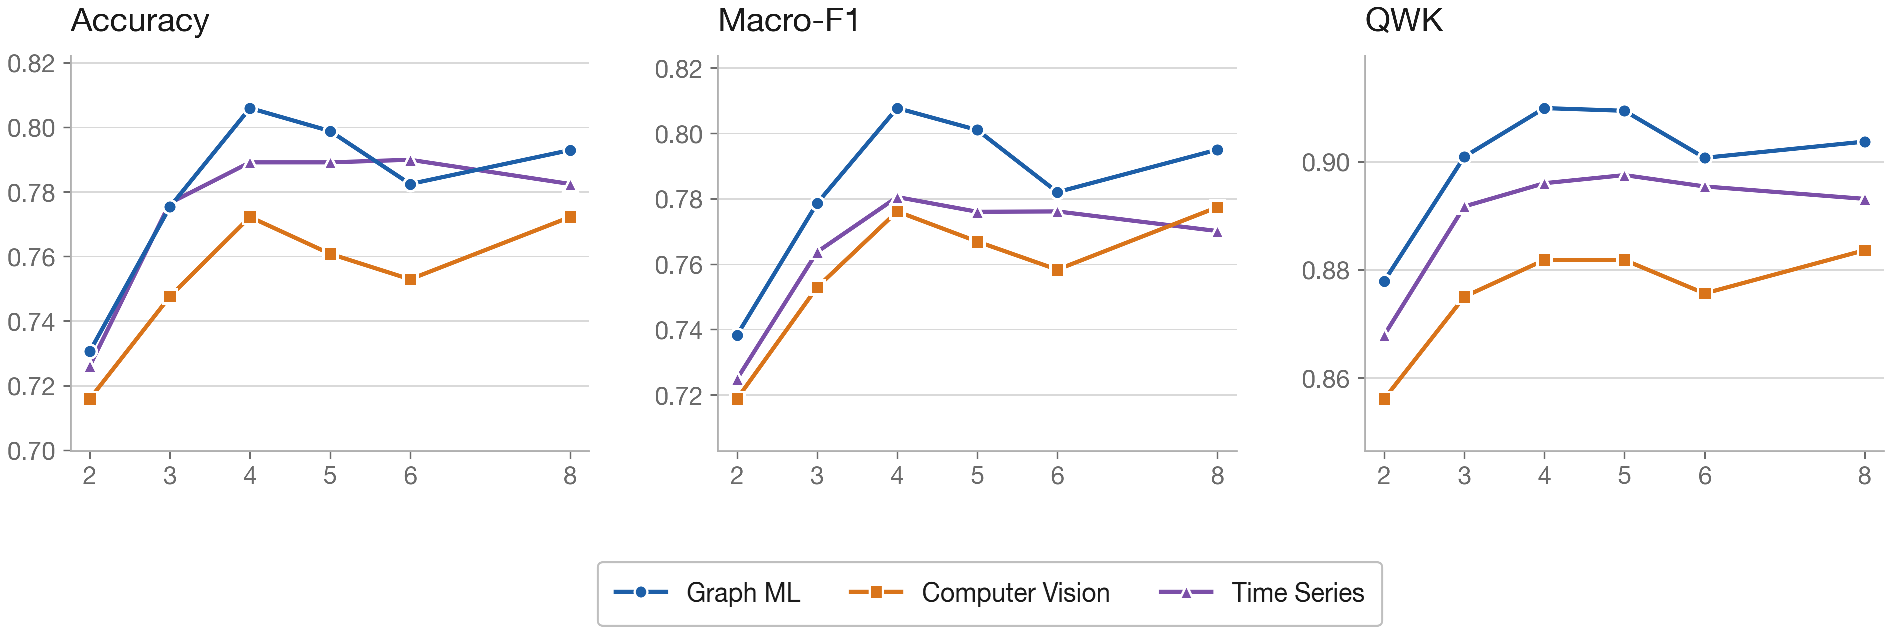
\includegraphics[width=\textwidth]{pic/param_sensitivity/topk.png}
\caption{Sensitivity to the evidence budget $K$ in the three domains. The
default is $K{=}5$, the checkpoint of Table~\ref{tab:panel-a}. $K$ is a padding
dimension, so the text reads the curves against the priors each setting
consumes.}
\label{fig:topk}
\end{figure}

\paragraph{Evidence budget: the ideas run out of priors before the model runs
out of capacity.}
Figure~\ref{fig:topk} varies $K$, the number of priors each idea contributes,
over $K=2,3,4,5,6,8$. Accuracy rises steeply from $K{=}2$ to $K{=}4$ ($0.731 \to
0.806$ on Graph ML, $0.716 \to 0.772$ on computer vision, $0.726 \to 0.789$ on
time series) and then flattens, with the same knee in all three domains. The
flattening comes from the evidence rather than from the model. Because every
sample is padded to exactly $K$ slots, the priors a setting consumes stop
growing once $K$ exceeds the candidates an idea carries, and the knee sits at
three to four consumed priors. Raising $K$ from 5 to 8 adds less than one
consumed prior, because about a third of the ideas carry six or more candidates
and fewer than one in seven carry eight or more.

\begin{figure}[h]
\centering
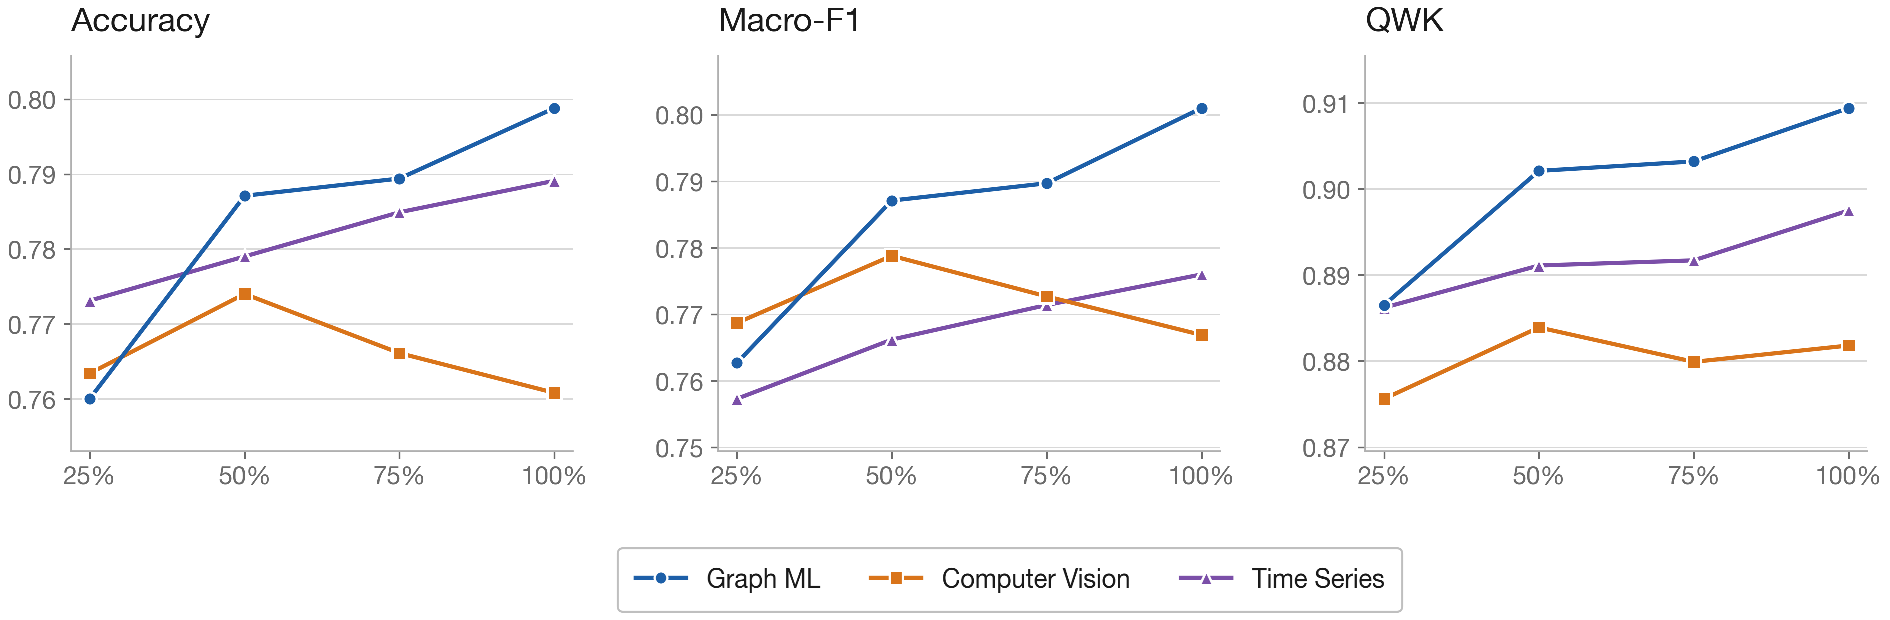
\includegraphics[width=\textwidth]{pic/param_sensitivity/train_frac.png}
\caption{Sensitivity to the amount of EGRD training data in the three domains.
Development and test sets stay fixed, and $100\%$ is the default.}
\label{fig:train-frac}
\end{figure}

\paragraph{Training-set size: more data helps across the board.}
Figure~\ref{fig:train-frac} varies the number of training ideas over $25\%$,
$50\%$, $75\%$ and $100\%$ of the training split, drawn as nested stratified prefixes so that
consecutive points add samples without reordering what came before. Macro-F1
rises steadily with the fraction on Graph ML ($0.7627 \to 0.8010$) and time
series ($0.7573 \to 0.7760$). Computer vision levels off after $50\%$ and ends
at $0.7669$ against a peak of $0.7788$, a gap of $0.012$. More training data
helps in most of the domains we measure, and the spread across the four
fractions stays small: accuracy moves by at most $0.039$ in any domain.

\begin{figure}[h]
\centering
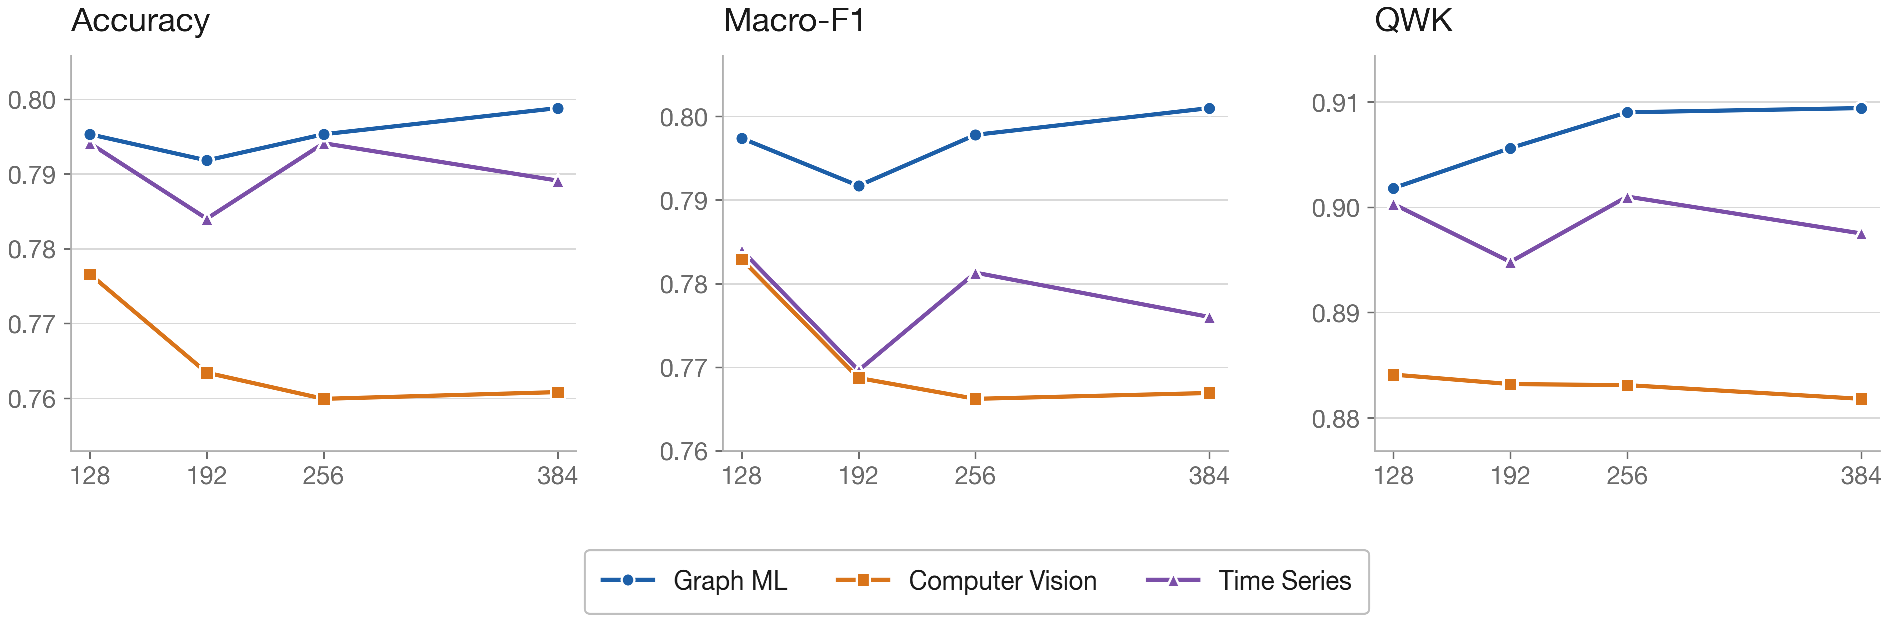
\includegraphics[width=\textwidth]{pic/param_sensitivity/max_length.png}
\caption{Sensitivity to encoder input length on the three domain test splits.
The default is 384, and every setting scores the same test ideas and labels.}
\label{fig:maxlen}
\end{figure}

\paragraph{Encoder input length: 128 tokens already cover the comparison.}
Figure~\ref{fig:maxlen} varies the encoder input length over 128, 192, 256 and
384 tokens. The four lengths separate the domains by little: no domain moves monotonically
with input length, and tripling the input moves Macro-F1 by at most $0.017$ in
any domain. At 128 tokens the encoder already covers the title-and-abstract
comparison for most target--prior pairs, so a longer window reads much the same
text and the curves stay flat. QWK is the flattest panel, spanning $0.0076$ on
Graph ML, $0.0023$ on computer vision and $0.0062$ on time series across the
four lengths, so the ordering the model produces is close to invariant to how
much of the text it reads. The flatness is consistent with the decomposition
reading a target and its priors through short unit-level comparisons rather than
through long spans of text.

\begin{table}[h]
\centering
\footnotesize
\setlength{\tabcolsep}{6pt}
\renewcommand{\arraystretch}{1.05}
\caption{Per-domain seed variability. Entries are sample standard deviations
across seeds 173, 174 and 175 with identical data, code and configuration.}
\label{tab:seed-noise}
\begin{tabular}{@{}l rrrrr@{}}
\toprule
Domain & Acc & Ma-F1 & QWK & MAE & High-F1 \\
\midrule
Graph ML & 0.0066 & 0.0050 & 0.0048 & 0.0067 & 0.0022 \\
Computer vision & 0.0040 & 0.0021 & 0.0032 & 0.0027 & 0.0037 \\
Time series & 0.0050 & 0.0045 & 0.0031 & 0.0051 & 0.0069 \\
\bottomrule
\end{tabular}
\end{table}

\paragraph{Seed stability: the reported model is not a selected seed.}
Table~\ref{tab:seed-noise} varies nothing but the random seed, running the
default configuration on seeds 173, 174 and 175 with identical data and code and
reporting the per-domain sample standard deviations. The spread is $0.004$--$0.007$ in accuracy and $0.002$--$0.005$ in Macro-F1, so
the headline numbers describe the configuration rather than one fortunate run,
and the three sweeps above should be read by the shape of a curve rather than by
the difference between adjacent points.